\documentclass[11pt,letterpaper]{article}
\usepackage[letterpaper, margin=1in]{geometry}
\usepackage[T1]{fontenc}
\usepackage[utf8]{inputenc}
\usepackage[english]{babel}
\usepackage{natbib,latexsym}
\bibliographystyle{plainnat}
\usepackage{graphicx}
\usepackage{hyperref}
\hypersetup{
    colorlinks=true,
    linkcolor=blue,
    filecolor=magenta,      
    urlcolor=cyan,
}
\title{Triplet Extraction from sentences}

\author{Sumith Baddam, Deepthi Raghu, John Stein, ... \\
  Affiliation
  {\tt \{srbaddam, draghu, jodstein, ...\}@iu.edu} \\}

\date{\today}

\begin{document}
\maketitle

\begin{abstract}
  In this paper we present an approach for extracting triplets from sentences using Json-NLP semantic relationship extractor and dependency parser. Triplet extraction is the processing of extracting subject-verb-object relationships from multiple sentences. This paper presents various traditional approaches previously used by others and evaluates our approach. We further compares our results with the results from traditional approaches. We would also discuss the evaluation procedure we followed and the challenges we faced in this project.
\end{abstract}

\section{Introduction}

Triplet Extraction is a crucial cog in the field of Natural Language Processing (NLP) and linguistics. It’s widely used for tasks such as Question Answering Systems, Machine Translation, Entity Extraction, Event Extraction, Named Entity Linking, Co-reference Resolution, Relation Extraction, etc.\\

A triplet represents a couple of entities and a relation between them. For example, (Damir Cavar, teach, NLP course) is a triple in which ‘Damir Cavar’ and ‘NLP course’ are the related entities, and the relation between them is ‘teach’. In this paper, we will focus on the extraction of these types of triples from a given text.\\

The main scope of this project is the triple extraction from sentences. Three relation types are explored.

\begin{itemize}
    \item Verb Relation: (subject, verb, object)
    \item Temporal Relation: (event, occurs after, event)
    \item Verb-Preposition Relation: (event, preposition, proposition object)
\end{itemize}

This problem requires understanding large corpora, which is an increasingly popular problem these days. In this report, we will discuss and explain some Natural Language Processing (NLP) techniques that we used to extract these relations from sentences and the different approaches used in particular by our team.


\section{Previous Work}
Our research about the previous work for this task exposed us to two different approaches. Traditional triplet extraction and open triplets extraction. In Traditional Extraction, the relations to be extracted are pre-defined. In Open Extraction, the relations are not pre-defined. The system is free to extract any relations it comes across while going through the text data. We also came across different methods from some of the research papers we read. Although many of these approaches involved building a neural model, we mainly focused on approaching the problem of triple extraction using a linguistic method (rule based extraction) because no labeled training data were available.

\subsection{Semantic Relationships: Get Structured Knowledge from Unstructured Text}
Let's have a look at text snippet, “Food Tutorials are better when directed by Wes Anderson. Bruce Lee's biopic, 'Little Dragon' to be directed by Shekhar Kapur.” \\

In the first sentence, we have two entities (“Food Tutorials” and “Wes Anderson”). These entities are related by the term “Directed”. Hence, (Wes Anderson, directed, Food Tutorials) is a triple.Similarly, we can extract relations from the other sentences as well, (Shekhar Kapur, directed, Little dragon). It turns out that we can get structured information based on the syntactic structure and grammar of the text, as illustrated in the example above.

\subsection{Different Approaches to Triplet Extraction}
In the previous section, we managed to easily extract triples from a few sentences. However, in the real world, the data size is huge and manual extraction of structured information is not feasible. Therefore, automating this information extraction becomes important.\\

There are multiple approaches to perform information extraction automatically. Let’s understand them one-by-one:
\begin{itemize}
    \item \textbf{Rule-based Approach:} We define a set of rules for the syntax and other grammatical properties of a natural language and then use these rules to extract information from text. 
    \item \textbf{Supervised:} Let’s say we have a sentence S. It has two entities E1 and E2. Now, the supervised machine learning model has to detect whether there is any relation (R) between E1 and E2. So, in a supervised approach, the task of relation extraction turns into the task of relation detection. The only drawback of this approach is that it needs a lot of labeled data to train a model.
    \item \textbf{Semi-supervised:} When we don’t have enough labeled data, we can use a set of seed examples (triples) to formulate high-precision patterns that can be used to extract more relations from the text.

\end{itemize}

\section{Approach}
For this task, we used NLTK, JSON-NLP and requests framework. We extract structured information from unstructured data (text data in our case). We’ve already seen that the information in text lies in the form of relations between different entities. \subsection{Subtree Matching for triplet extraction}
Our methodology is similar to subtree matching for relation extraction.\\

The simple rule-based methods work well for information extraction tasks. However, they have a few drawbacks and shortcomings. We have to be extremely creative to come up with new rules to capture different patterns. It is difficult to build patterns that generalize well across different sentences. To enhance the rule-based methods for relation/information extraction, we should try to understand the dependency structure of the sentences at hand. We use JSON-NLP API for getting the dependency structure of the sentence. From the output of the API, we try to find interesting relationships. \\

For example, let's consider the sentence to be, “Tableau was recently acquired by Salesforce.” Output from the API is <Image>\\

If you look at the entities in the sentence – Tableau and Salesforce – they are related by the term ‘acquired’. So, the pattern I can extract from this sentence is either “Salesforce acquired Tableau” or “X acquired Y”.\\

Now consider another statement, “Careem, a ride-hailing major in the middle east, was acquired by Uber.” Output from the API is <Image>\\

From the graph, all we have to check is which dependency paths are common between multiple sentences. This method is known as Subtree matching. We will just consider the common dependency paths and extract the entities and the relation (acquired) between them. Hence, the relations extracted from these sentences are:
\begin{itemize}
    \item Salesforce acquired Tableau
    \item Uber acquired Careem
\end{itemize}

After extracting a basic subject - verb - object extracted from a single sentence by the above approach, we had to handle compounds such as adjectives and modifiers. Also, we had to handle sentences with multiple subject/verb/object occurrences, define a particular output structure and handle reading multiple files containing multiple sentences. In addition to this, event ordering also had to be included. The various experiments done to achieve these results have been described in the next section. 

\section{Experiments (draghu)}
This section discusses the experiments and implementation done by Deepthi Raghu.

\noindent \newline
One of the approaches for rule-based triple extraction was to perform dependency parsing by writing rules to identify compounds such as adjectives and modifiers from the dependency tree. The rules are specifically based on the 'tokenlist' and the 'dependency' parts of the JSON from the NLP-API. 

\subsection{Method 1}
In this approach, the input is a list of files containing multiple sentences line by line. The output will be a list of JSONs corresponding to each sentence in the input files. \\
\noindent
For example, if the input is a file containing two sentences:

"Mary marinated the chicken." 

"John cooked the chicken."

\noindent \newline
Then the output will be:

\{'sentence': 1, 'event': 1, 'subject': 'Mary', 'verb': 'marinate', 'object': 'chicken'\}

\{'sentence': 2, 'event': 2, 'subject': 'John', 'verb': 'cook', 'object': 'chicken'\}

\noindent \newline
Explanation of output:
\begin{itemize}
    \item The sentence key in the output JSON provides a reference to the sentence number in the input sentence file.
    
    \item The event key in the output JSON indicates the event ordering i.e, the ordering of the predicates.
    
    \item The subject, verb and object keys indicate the triples that have been extracted.
\end{itemize}
The rules were extended as and when new scenarios and variations of the triples have to be handled.
Below are some example sentences from file15.txt in webanno to show the different variations handled:
\begin{enumerate}
    \item
    \textbf{Sentence:} Prepare the cake mixes according to the package directions. \newline
    \textbf{Variation in triple:} This sentence has a compound object 'cake mixes'.
    \newline
    \textbf{Extracted output:} 
    
    \{'sentence': 1, 'event': 1, 'subject': '<imperative-chef>', 'verb': 'prepare', 'object': 'cake mix'\}
    \newline
    \textbf{Inference from output:} 
    An important point to note is that in sentences that do not have a subject, the subject is replaced with "<imperative-chef>". In this particular example, the output shows that the compound object "cake mix" has been extracted successfully.
    
    \item
    \textbf{Sentence:} Stir to combine, then add the milk, cream and butter.
    \newline
    \textbf{Variation in triple:} This sentence has a multiple objects - milk, cream, butter
    \newline
    \textbf{Extracted output:} 
    
    \{'sentence': 1, 'event': 1, 'subject': '<imperative-chef>', 'verb': 'add', 'object': 'milk'\}
    
    \{'sentence': 1, 'event': 1, 'subject': '<imperative-chef>', 'verb': 'add', 'object': 'cream'\}
    
    \{'sentence': 1, 'event': 1, 'subject': '<imperative-chef>', 'verb': 'add', 'object': 'butter'\}
    
    \textbf{Inference from output:} 
    Whenever there are multiple subjects/verbs/objects, this approach will naively produce all combinations of triples. In this case, the three objects, milk, cream and butter have been identified and put into three different triples. Since all the extracted triples are from the same sentence, the sentence key remains unchanged.
    
    \item
    \textbf{Sentence:} Cover and cook until cauliflower begins to soften, about 4 minutes.
    \newline
    \textbf{Variation in triple:} This sentence has a multiple verbs - cover, cook and it has no object
    \newline
    \textbf{Extracted output:} 
    
    \{'sentence': 1, 'event': 1, 'subject': 'cauliflower', 'verb': 'cover', 'object': '<None>'\}
    
    \{'sentence': 1, 'event': 2, 'subject': 'cauliflower', 'verb': 'cook', 'object': '<None>'\}
    
    \textbf{Inference from output:} 
    Whenever there are multiple subjects/verbs/objects, this approach will naively produce all combinations of triples. In this case, the two verbs cover and cook have been identified and put into two different triples. Also, since this sentence does not have an object, the object is replaced with '<None>'. Another point to note here is that since there are two verbs in this sentence, the event changes accordingly, capturing the order in which the actions occurred.

\end{enumerate}

\noindent
In this manner, multiple files containing multiple sentences line by line is processed to produce an output JSON. 

\noindent \newline
\textbf{Steps to run the code for this experiment:}
\begin{itemize}
    \item Run the python code \textbf{extract\_triples\_draghu.py} using the command:
    
    \textbf{python extract\_triples\_draghu.py file1.txt file2.txt ...}
    
    where, file1.txt, file2.txt .. are the input files
    
    \item After the execution of code, the result is generated in the file \textbf{method1\_relations\_draghu.txt}
\end{itemize}

\subsection{Method 2}
\noindent
In order to standardize the outputs of all the experiments, the graph.py code was utilized to give a graph object as the output. To incorporate this output format, the existing code \textbf{extract\_triples\_draghu.py} was modified to \textbf{extract\_triples\_graph\_draghu.py} and two relations were constructed:

\begin{itemize}
    \item Triples (Subject, Verb, Object)
    \item Event relation (Event2 occurs\_after Event1)
\end{itemize}

\noindent
The graph.py enabled us to produce two types of results:
\begin{enumerate}
    \item A graph object with nodes and edges represented as a JSON 
    \item A line by line relation extraction
\end{enumerate}
\noindent
Below is an example:
\noindent \newline
\textbf{Sentences:} 

Prepare the cake mixes according to the package directions.

Stir to combine, then add the milk, cream and butter.

\noindent 
\textbf{Extracted output1 : A graph object represented as a JSON } 
\newline

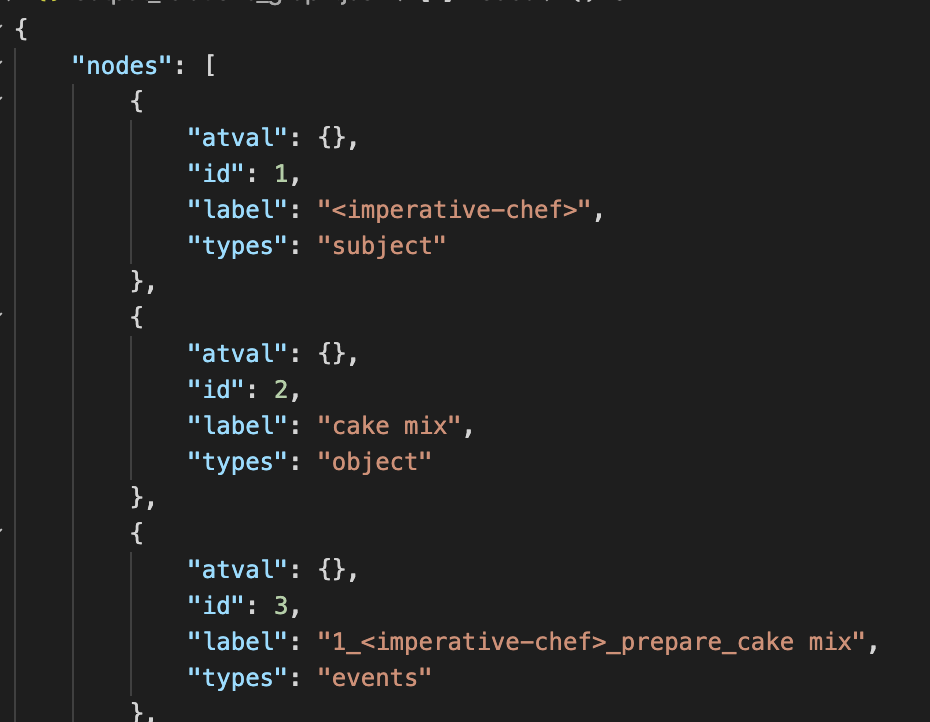
\includegraphics[width=9cm, height=7.75cm]{graph_obj1.png}
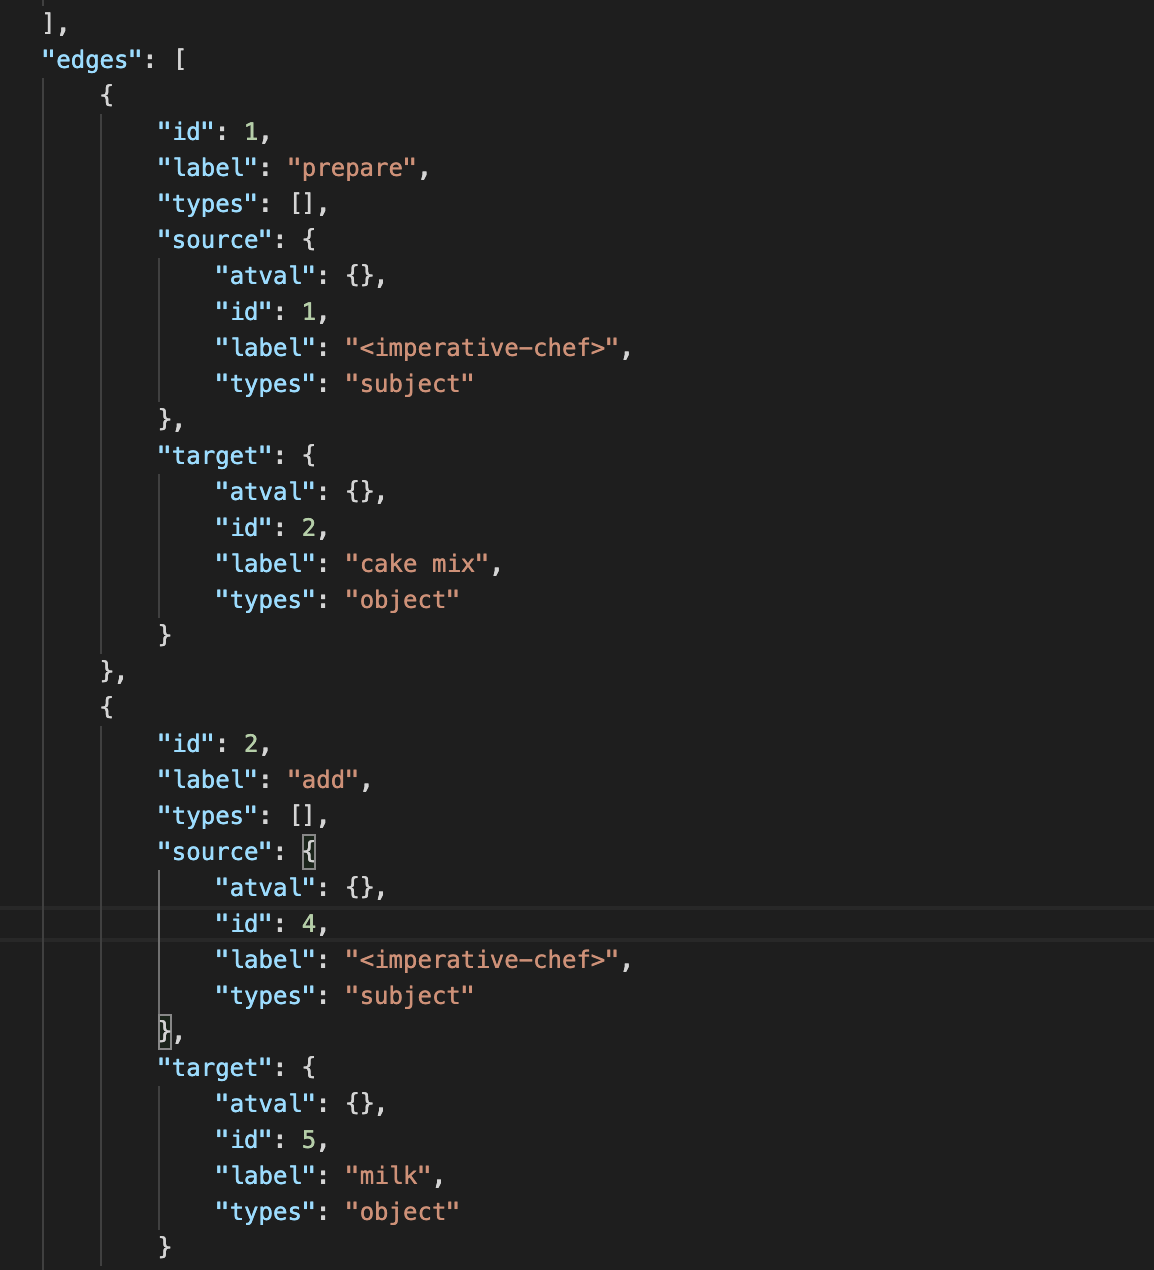
\includegraphics[width=9cm, height=7.75cm]{graph_obj2.png}

\noindent
\textbf{Extracted output2 : A line by line relation extraction } 

\begin{flushleft}
\{'source': '<imperative-chef>', 'relation': 'prepare', 'target': 'cake mix'\}

\{'source': '<imperative-chef>', 'relation': 'add', 'target': 'milk'\}

\{'source': '<imperative-chef>', 'relation': 'add', 'target': 'cream'\}

\{'source': '<imperative-chef>', 'relation': 'add', 'target': 'butter'\}

\{'source': '2\_<imperative-chef>\_add\_milk', 'relation': 'occurs\_after', 'target': '1\_<imperative-chef>\_prepare\_cake mix'\}

\{'source': '3\_<imperative-chef>\_add\_cream', 'relation': 'occurs\_after', 'target': '2\_<imperative-chef>\_add\_milk'\}

\{'source': '4\_<imperative-chef>\_add\_butter', 'relation': 'occurs\_after', 'target': '3\_<imperative-chef>\_add\_cream'\}

\end{flushleft}
\noindent 
\textbf{Inference from output1:} 

In the graph object, Subjects, Objects and Events are constructed as nodes. An edge is drawn in two cases:
\begin{enumerate}
    \item Edge over a verb, connecting a subject and an object to capture triple relations
    \item Edge over "occur\_after", connecting two events to capture event relations
\end{enumerate}
\noindent 
\textbf{Inference from output2:} 

This output gives a line by line relation extraction. It extracts two relations:

\begin{itemize}
    \item Triple relations like \{'source': '<imperative-chef>', 'relation': 'add', 'target': 'milk'\}
    \item Event relations like \{'source': '3\_<imperative-chef>\_add\_cream', 'relation': 'occurs\_after', 'target': '2\_<imperative-chef>\_add\_milk'\}
    
\end{itemize}
\noindent \newline
Also, in this experiment, the event ID has been generated by concatenating the verb ID from its corresponding graph node with with subject, verb and object as "verbID\_subject\_verb\_object to get a unique event ID.

\noindent \newline
\textbf{Steps to run the code for this experiment:}
\begin{itemize}
    \item Run the python code \textbf{extract\_triples\_graph\_draghu.py} using the command:
    
    \textbf{python extract\_triples\_graph\_draghu.py file1.txt file2.txt ...}
    
    where, file1.txt, file2.txt .. are the input files
    
    \item After execution of the code, the graph object (output1) is generated in
    
    \textbf{method2\_relations\_graph\_draghu.json} and the line by line relation extraction (output2) is generated in \textbf{method2\_relations\_triples\_draghu.txt}
\end{itemize}
\newpage

\section{Experiments (jodstein)}\label{jodstein_experiments}

This section discusses the evolution of approaches and experiments undertaken by John Stein.

\subsection{A brief discussion of Neural approaches}
The initial approach considered was to build a neural network, or set of neural networks, trained to extract various relation types from a sample text.  The primary advantage of a neural network approach is that they can be arbitrarily complex (number of hidden layers, number of nodes per hidden layer, any architecture) and so are able to learn very rich (semantically-speaking) representations of inputs and produce outputs (extractions, classifications) that would not be achievable through lexical approaches.  However, a neural approach implies several pre-requisites and intermediate tasks:

\begin{itemize}
    
    \item Labeled Data - Neural networks must have access to labeled data so that errors can be identified and their tensor values can be correspondingly adjusted.  The data available to the relation extraction group was not labeled, and was relatively small (in comparison to many other neural network datasets).  These constraints would have resulted in having to annotate relations for the entire dataset, creation of negative (false) relations to aid in the training process, and placing limitations on the number of relation types that could be extracted.
    
    \item Architecture - The architecture plays a central role to a network's performance against the assigned task.  For example, recurrent networks have the ability to carry information from previous inputs and network state into subsequent inputs, which is particularly well suited for linear sequential input types.  Language is a little more complicated than that, so more complicated structures such as Long Short-Term Memory (LSTM) \cite{article}, Gated Recurrent Units (GRU) \cite{DBLP:journals/corr/ChoMGBSB14}, or Attention \cite{bahdanau2014neural} are likely to perform better.
    
    \item Input and Data Representation - It is best practice when using neural models for NLP tasks to represent the input text as a feature vector vice raw text.  This is because the words, characters, and character encodings aren't defined in a way that is at all relevant to the semantic meaning of the text.  Multiple approaches for encodings have been used with success, including some popular examples such as Word2Vec \cite{mikolov2015computing}, FastText \cite{DBLP:journals/corr/JoulinGBDJM16}, and Bidirectional Encoder Representations from Transformers (BERT) \cite{DBLP:journals/corr/abs-1810-04805}.  
    
    \item External Data - Features derived from annotations (parts of speech, named entities, dependencies, constituency, etc.) may provide valuable in the automated learning task, so an encoded representation would need to be learned.  Further, external data sources such as ontologies, knowledge graphs, or databases may help a great deal in performance of the neural model, if they can be leveraged.  FrameNET, in particular, contains very powerful information about semantic concepts, how they are most often presented in text, and what their argument structure looks like.  Use of FrameNET, or any of these external data, in a neural model might be accomplished in a way similar to word embeddings mentioned above but, instead of training the embeddings to predict co-occurrence of other words, the embeddings would be trained to classify the conceptual frame being represented by the sentence or word span.
    
\end{itemize}

\subsection{The Implemented Approach}

This section discusses the approach and associated experiments undertaken by John Stein.  Code for these experiments can be found in \texttt{ML4NLP/group3/} as \texttt{extract\_jodstein\_v0.py}, or previous committed versions as \texttt{extract\_jodstein.py}.  File can be run from the ML4NLP/group3 folder in the console using \texttt{python extract\_jodstein\_v0.py <path-for-file(s)>}.

\begin{enumerate}

    \item Constituency Parsing - The first experiments were based on a constituency parse of the sentence.  The thinking behind using constituency parsing was that, for complex sentences, an entire phrase or clause may be playing the role of semantic subject, verb, or object in the context of a given sentence.  The theory behind following the constituency parse was that a recursive algorithm could inspect clauses and phrases for arbitrarily-complex sentences, and could build some context representation from the top-level on down into the recursion so as to enable more powerful entity and relation extraction at the deepest levels.  This is similar to the notion of tail recursion where an environment is continuously built up through the recursion process and when actual extraction occurs, it happens in the presence of a well-structured trace through the constituency parsing, ignoring sentence elements that are not a part of that trace.  This approach turned out to be fraught with complicating factors, including (a) constituency labels don't themselves reveal even the lexical subject/object parts of a sentence, much less the semantic parts, and (b) the representation of context down through the recursion remained a task-too-far without the benefit of embeddings or semantically-encoded represetnations.  This work can be viewed under commit \texttt{27bfd29394075086c777625976caadb525404748}, but was never complete to the point it would run.
    
    \item Dependency Parsing - The next approach taken, based on feedback from the professor, was a Dependency-based approach.  This approach is much simpler because the subjects and objects of verbs are already labeled/annotated.  However, the successful extraction of relations is inextricably tied to the quality of the dependency annotations.  Initial dependency-based success simply extracted verb-relations using the verb token as the relation, dependent tokens labeled with \texttt{nsubj} that were governed by that verb as the subjects, and dependent tokens labeled with \texttt{dobj} that were goverened by the verb as the objects.  The next success was to successfully trace any subject or object token to include any other token with which it shared a compound chunk.  Further, many verbs have multiple subjects and/or multiple objects via conjunctions.  To handle this, the algorithm permutates over every combination of subject and noun around the verb that serves as the governer for both.  Hence, all verbs resulted in $ \mid subjects \mid \times \mid objects \mid $ verb-relations.  Show below is an example sentence with extracted relations:
    
        \begin{verbatim}
            "This vegan salad makes a healthy and filling meal, providing 4 of
            your 5-a-day."
            
            Extracted: (vegan salad,  make,  meal)
        \end{verbatim}
        
    This approach produced around 100 relations from the Corpus, and can be viewed/run under commit \texttt{86aea17093c51cf51fcb3669de0750fc1f413766}.
    
    \item Temporal Relations and Dummy Values - The next step taken was to include the notion of event timelines.  This was at the specific request of Group 4, who wanted to demonstrate some event-based knowledge representation in their graph work.  To capture event timelines, the notion of an event must first be established.  Essentially, the approach was to create an event node/entity for each verb-relation and embed the Edge.id from the corresponding verb-relation into the event node's label.  Next, the algorithm keeps a short term memory containing the set of events corresponding to the last verb encountered. Finally, for every new verb encountered, the algorithm creates \texttt{occurs\_after} temporal-relations between the events associated with the current verb and those in short term memory.  The short term memory is cleared between documents since there is no temporal relationship between entirely separate text sources.  Also, the group noticed that any verbs that didn't have both a noun subject and a direct object were not being captured.  Since the corpora consisted of recipes, many of the statements were imperative without a subject.  To solve this, the group decided to create a dummy entity \texttt{<imperative-chef>} to serve as the subject for imperative statements, and a dummy entity \texttt{<None>} to serve as the direct object when one wasn't present.  Show below is an example sentence with extracted relations:
    
    \begin{verbatim}
        "With the mixer on low speed, add 1/2 cup of the flour at a time, 
            waiting for each addition to be fully incorporated before 
            adding more."
            
        Extracted: (<imperative-chef>,  add,  cup)
        Extracted: (<imperative-chef> ,  wait ,  <None>)
        Extracted: (5009_<imperative-chef>_wait_<None>,  occurs_after,  
            5005_<imperative-chef>_add_cup)
        Extracted: (<imperative-chef>,  be,  <None>)
        Extracted: (5012_<imperative-chef>_be_<None>,  occurs_after,  
            5009_<imperative-chef>_wait_<None>)
        Extracted: (<imperative-chef> ,  add ,  more)
        Extracted: (5014_<imperative-chef>_add_more,  occurs_after,  
            5012_<imperative-chef>_be_<None>)
    \end{verbatim}
    
    
    The addition of Temporal relations and other dummy values resulted in around 300 relations from the Corpus, and can be viewed/run under commit \texttt{3ea35b27eb3aa289fbc5a0f5bdaf06e053178131}.
    
    \item Prepositional Relations - The next step taken was to include prepositional relations.  This task was somewhat straightforward to implement, having become familiar with how to navigate the dependency tree.  Essentially, after defining verb-relations, the algorithm gathers all tokens (prepositions) that are governed by that same verb under a \texttt{prep} dependency type and iterates on each.  For each preposition, a lit of tokens dependent on that preposition under a \texttt{pobj} dependency type (with compounds) are then collected as objects for that preposition.  Finally, a set of relations are created with the events corresponding to the verb as the sources, the prepositions as the relation labels, and the propositions' objects as the relation targets, permutated over all combinations as before.  Show below is an example sentence with extracted relations:
    
    \begin{verbatim}
        "Make bread crumbs by placing the bread in the work bowl of a food 
            processor and processing until finely ground."
            
        Extracted: (<imperative-chef>,  make,  <None>)
        Extracted: (4968_<imperative-chef>_make_<None>,  occurs_after,  
            4966_<imperative-chef>_remain_<None>)
        Extracted: (<imperative-chef>,  place,  bread)
        Extracted: (4970_<imperative-chef>_place_bread,  occurs_after,  
            4968_<imperative-chef>_make_<None>)
        Extracted: (4970_<imperative-chef>_place_bread,  in,  work bowl)
        Extracted: (4970_<imperative-chef>_place_bread,  until,  grind)
        Extracted: (<imperative-chef>,  process,  <None>)
        Extracted: (4974_<imperative-chef>_process_<None>,  occurs_after, 
            4970_<imperative-chef>_place_bread)
    \end{verbatim}
    
    This approach resulted in around 5,000 relations from the Corpus, and can be viewed/run under commit \texttt{f636830a9751e43732a27ede19d0ac02b64f45a1}.
    
    \item Dependency with Verb-as-Entity - The final significant change to the relation extractor was to regard verb tokens as entities, rather than as relations.  As stated above in the Temporal Relations step, the current method for linking a verb-relation to an event was to include the verb-relation identification number in the event label.  That hack may serve the immediate purpose, but is counter to the purist aspects of knowledge management.  An improved approach is recognize that each verb is an entity in its own right, representing an activity, action, or being, and doesn't get its meaning from any one event instance.  So, after creating an entity for each verb encountered (the idea of the verb) as well as an event for each verb encountered (the instance of a verb being involved in a specific event), it is possible to add the relation \texttt{involves\_verb} which ties the verb to the event.  In this way, the event also becomes the center for all subjects, objects, and prepositional statements.  Afterall, these other entities are only linked to each other through the event in which they all had a role.  This change was implemented late in the project, but is not planned for processing by the graph subgroup due to the fundamental change in the way even the most basic relations are captured.  Show below is an example sentence with extracted relations:
    
    \begin{verbatim}
        "Sprinkle the cream of tartar over the egg whites and continue to 
            beat until they hold a soft peak."
            
        Extracted: (34_Sprinkle, involves_verb, Sprinkle) 
        Extracted: (34_Sprinkle, has_object, cream)
        Extracted: (37_continue, involves_verb, continue)
        Extracted: (37_continue, occurs_after, 34_Sprinkle)
        Extracted: (39_beat, involves_verb, beat)
        Extracted: (39_beat, occurs_after, 37_continue)
        Extracted: (41_hold, involves_verb, hold)
        Extracted: (41_hold, has_subject, -PRON-)
        Extracted: (41_hold, has_object, peak)
        Extracted: (41_hold, occurs_after, 39_beat)
    \end{verbatim}
    
    
    This approach resulted in around 6,100 relations from the Corpus, and can be viewed/run under commit \texttt{c002c099852dce47468a7d366e614f4514e9f146} as \texttt{extractor\_jodstein\_v1.py} (the previous approach continues to be maintained as \texttt{extractor\_jodstein\_v0.py}).

\end{enumerate}

\section{Evaluation}

This is how we evaluated our work, presenting the evaluation scores in comparison to previous projects...

Describe manual evaluation methodology: (1) look at sentence, (2) observe extracted triplets, (3) observe annotations in context of how our rule-based approach is programmed.  Walk through several examples.



\section{Discussion}

\subsection{Knowledge Graph vs Ontology}\label{ont_vs_kg}

Current popular opinion \cite{science_where_2018, schrader_whats_2020} has the definitions for ontology and knowledge graph loosely differentiated.  The key difference, it would appear, has ontologies capturing schema, while knowledge graphs capture facts.  Stated another way, an ontology may be the tool of choice to capture or define how a universe of relevant entities (classes, attributes, relations, rules, etc.) are related to one another, while a knowledge graph may be the tool of choice to capture factual knowledge in a structured way as it is encountered in the real world.  The difference here is not clear in all cases.  Take a simple example: "The police officer ordered a custard-filled donut."  Is "police officer" an instance of "person::employee::law\_enforcement", or is it a concept in its own right.  A common approach is to treat "police officer" as an instance of an existing entity until such time that it becomes necessary/desirable to reason about "police officer" in relation to other entities.  From an ontological perspective, the schema continues to be defined at lower levels as more granular schemas and relations emerge from real data.  From a knowledge graph perspective, there must be an expectation that the knowledge graph is re-defined when new schemas emerge and subsequently used to better organize and reason over the facts captured in real data.


\subsection{Everything as Entities}

One of the challenges encountered during the progression of various approaches to triple extraction relates to pre-suppositions about what the resulting relation set might contain, and how one might want to reason over those relations.  More specifically, the initial expectation among many in the class was that the relations extracted would always be of the form (subject, verb, object).  While it is true that this was the initial approach (easiest to accomplish), this expectation resulted in some implementation decisions on the part of group 3 and the API group which may constrain the versatility and power of the knowledge graph representation.  For example, as discussed in Section \ref{jodstein_experiments} above, the initial choice to extract verbs as the relation versus as an independent entity constrained the resulting knowledge graph in several ways:

\begin{enumerate}
    \item Could not define temporal relations between verbs
    \item Could not define preposition relations between verbs and preposition objects
    \item Could not reason about verbs as concepts (identifying all the objects of 'chop')
    \item Could not truly link verb-relations to the concept of an event (using graph methodology)
\end{enumerate}

Although some of these constraints were overcome, the means by which they were overcome involve, in some cases, implicit knowledge about how the relations were constructed and how to interpret them.  In other words, the reasoning engine relies on implicit knowledge about the relations it is reasoning over (e.g. the verb-relation id embedded in event labels or knowledge that verb-relation ids are representative of their temporal placement in the text).  Through this exercise, a couple of important lessons emerged which build on the concepts discussed in Section \ref{ont_vs_kg}.  Firstly, a pattern emerges wherein as the desire to learn and reason over more abstract and semantically-rich concepts and notions increases, so does the necessity to represent these higher-level concepts as entities.  This is necessary because in order to capture more subtle nuances between texts, the reasoning engine must operate at higher levels of semantic meaning and/or abstraction, and so relations must be drawn at those levels to enable that reasoning.  Secondly, a design requirement for the reasoning engine should be that it can reason over arbitrary relation types.  Obviously the queries for the engine will likely be specific to the set of relation types that exist in the knowledge graph, but the engine logic should not be.




\subsection{Conclusion}

Some conclusion...


% the bibliography
\bibliography{main}


\end{document}
